% !TEX root = ../../../../temp_manuscript.tex

\chapter[Differences in spatial distribution between WHO 2016 low-grade glioma molecular subgroups][LGG location molecular subgroups]{Differences in spatial distribution between WHO 2016 low-grade glioma molecular subgroups}\label{chap:LGGLocation}



\begin{ChapterAbstract}
    \textbf{Background:} Several studies reported a correlation between anatomic location and genetic background of \cglspl{LGG}.
    As such, tumor location may contribute to presurgical clinical decision-making.
    Our purpose was to visualize and compare the spatial distribution of different \cgls{WHO} 2016 gliomas, frequently aberrated single genes and DNA copy number alterations within subgroups, and groups of postoperative tumor volume.

    \textbf{Methods:}
    Adult grade II glioma patients (\cgls{WHO} 2016 classified) diagnosed between 2003 and 2016 were included.
    Tumor volume and location were assessed with semi-automatic software.
    All volumes of interest were mapped to a standard reference brain.
    Location heatmaps were created for each \cgls{WHO} 2016 glioma subgroup, frequently aberrated single \cglspl{CNV}, as well as heatmaps according to groups of postoperative tumor volume.
    Differences between subgroups were determined using voxelwise permutation testing.

    \textbf{Results:}
    A total of 110 \cgls{IDH} mutated astrocytoma patients, 92 \cgls{IDH} mutated and \acl{1p19qcodel} oligodendroglioma patients, and 22 \cgls{IDH} wild-type astrocytoma patients were included.
    We identified small regions in which specific molecular subtypes occurred more frequently.
    \cgls{IDH}-mutated \cglspl{LGG} were more frequently located in the frontal lobes and \cgls{IDH} wild-type tumors more frequently in the basal ganglia of the right hemisphere.
    We found no localizations of significant difference for single genes/\cglspl{CNV} in subgroups, except for loss of 9p in oligodendrogliomas with a predilection for the left parietal lobes.
    More extensive resections in \cgls{LGG} were associated with frontal locations.

    \textbf{Conclusions:}
    \cgls{WHO} low-grade glioma subgroups show differences in spatial distribution.
    Our data may contribute to presurgical clinical decision-making in \cgls{LGG} patients.

    \publishedas{wijnenga2019differencesLGG}
\end{ChapterAbstract}

\section{Introduction}
Classification of diffuse gliomas is based on histological and molecular criteria according to the 2016 \cgls{WHO} classification of tumors of the central nervous system \autocite{louis2014international}.
Three major subtypes of diffuse \cgls{LGG} (grade II)  are recognized based on testing of 2 molecular markers: mutations of \cgls{IDH} 1 or 2 gene and combined deletion of chromosomal arms 1p and 19q.
Next to the \cgls{WHO} classification, (eloquent) location, size, presence of contrast enhancement, and delineation of the tumor margins on \cgls{MR} imaging are important prognostic factors \autocite{pignatti2002prognostic, jakola2012low, capelle2013spontaneous, chang2008preoperative}.

Previous studies suggest that the anatomic location of a glioma is correlated with the molecular background of the tumor \autocite{stockhammer2012idh1, goze2009lack, laigle2004correlations, metellus2010absence}.
If so, tumor location may contribute to presurgical clinical decision-making and may provide a noninvasive marker for prediction of molecular subtype.
However, current evidence to support this is mainly derived from relatively small series which are often single molecular marker studies  \autocite{stockhammer2012idh1, goze2009lack, laigle2004correlations, metellus2010absence}.
For example, it was shown that loss of 1p is associated with a more frequent location in the frontal lobes and that \acl{1p19qcotion} is absent in insular tumors \autocite{goze2009lack, laigle2004correlations}.
In a series of 47 patients, \citeauthor*{metellus2010absence} showed that \cgls{IDH} wild-type \cgls{LGG} are preferentially located in the insular region.
We recently reported on a cohort of resected LGG samples, wherein we found that IDH wild-type tumors were more often located in eloquent areas \autocite{wijnenga2017impact}.
In that study, just as in many other previous studies on glioma location, we used the cerebral lobes as the location description factor, which is not accurate.
A recent study by \citeauthor*{tejada2018voxel} showed a location predilection for \cgls{IDH}-mutated tumors in the frontal lobes in the rostral extension of the lateral ventricles.
Despite these data, no large series have been described that visualize the anatomic location of \cgls{WHO} 2016 LGG subtypes in a voxel-based manner.
As the \cgls{WHO} 2016 criteria are more objective than the previous \cgls{WHO} 2007 criteria and result in a more refined and prognostic classification of tumors, it is possible that the spatial distributions of different \cgls{WHO} 2016 glioma subtypes are more distinct than previously shown for the classical histopathological classification \autocite{larjavaara2007incidence}.

Previously, we investigated the impact of extent of resection in \cgls{WHO} 2016 classified \cgls{LGG} and assessed tumor volume location and volume in a semiautomatic manner \autocite{wijnenga2017impact}.
We used this cohort in the present study to visualize the spatial distribution of different \cgls{WHO} 2016 \cgls{LGG} subtypes, by creating voxel-based probability maps of tumor location for every subtype.
Using this cohort also enabled us to visualize spatial distributions of \cglspl{LGG} according to the extent of resection.
These maps might be helpful in presurgical decision-making.

\section{Methods}
\subsection{Patient selection}
Adult patients (age $\geq$ 18 years) with histopathologically confirmed supratentorial grade II glioma were included.
Patients and samples were previously described in a study investigating the extent of resection in grade II glioma \autocite{wijnenga2017impact}.
All patients were treated in a single institute between 2003 and 2016, The Brain Tumor Center at Erasmus MC Cancer Institute in Rotterdam, the Netherlands.
The study was approved by the medical ethics committee of Erasmus MC and conducted according to national and European regulations.

\subsection{Image Acquisition and Processing}
We used the preoperative \cgls{MR} scans that were available from a routine clinical setting.
\cgls{MR} sequence protocols varied per patient, as patients were diagnosed in several centers without the use of a uniform tumor \cgls{MR} imaging protocol.
For inclusion in this study, at least a \cgls{FLAIR} or \cgls{T2} sequence needed to be available.
We did not use inclusion or exclusion criteria for voxel size and/or slice thickness.
We segmented preoperative and postoperative glioma lesions on MR imaging in a semiautomated fashion with the SmartBrush tool that is incorporated in Brainlab Elements (version 2.1.0.15).
With this tool, a three-dimensional (3D) \cgls{VOI} can be created by manually segmenting the lesion on 2 perpendicular slices, from which the software calculates a full 3D \cgls{VOI}, which was manually adjusted where necessary.
We used the \cgls{FLAIR} sequence when available (3D where possible); otherwise, the conventional \cgls{T2} sequence was used for segmentation.
All tumor-related \cgls{T2} and \cgls{FLAIR} signal abnormalities were included in the segmentation.
The \cgls{T2} and \cgls{FLAIR} images of all patients were affinely registered (preserving parallel lines and planes) to the \cgls{MNI} \cgls{ICBM} 152 nonlinear T2w atlas \autocite{fonov2011unbiased, fonov2009unbiased} and the 3D \cglspl{VOI} were transformed accordingly for further analysis.
We registered all \cgls{MR} images using an automated algorithm based on maximization of mutual information \autocite{klein2009adaptive}, as implemented in the open-source SimpleElastix software (version 9dfa8cb) \autocite{marstal2016simpleelastix}
All registrations were manually checked to assure proper alignment with the atlas, and adjusted where necessary.

\subsection{DNA Extraction and Next-Generation Sequencing}

Areas with high tumor content were manually macrodissected from \cgls{FFPE} tissue slides as described previously \autocite{wijnenga2017impact}.
We used a targeted \cgls{NGS} panel to classify samples according to the \cgls{WHO} 2016 criteria, using an Ion Torrent Personal Genome Machine or Ion S5XL (Life Technologies).
The panel assesses mutational status of \cgls{IDH}1/2, TP53, FUBP1, PTEN, CIC, CDKN2A, NOTCH1, ATRX (whole gene) and hotspots of EGFR (exon 3 + 15), H3F3A (exon 2), PIK3CA (exon 10 + 21), BRAF (exon 11 + 15), and also \cglspl{CNV} of chromosome 1, 7, 9, 10, 12, and 19.
TERT promoter mutations (C228T and C250T) were assessed in a separate assay (SnaPshot).
Detailed methods were described previously \autocite{wijnenga2017impact, wijnenga2018prognostic}.

The following criteria for molecular classification were used:

\begin{itemize}

\item Oligodendroglioma: \cgls{IDH}1 or \cgls{IDH}2 mutated and loss of heterozygosity consistent with co-deletion of the entire 1p and 19q chromosomal arms.

\item \cgls{IDH} mutated astrocytoma: \cgls{IDH}1 or \cgls{IDH}2 mutated.

\item \cgls{IDH} wild-type astrocytoma, with molecular features of glioblastoma (according to recent cIMPACT-NOW update 3,18  in further text named as "\cgls{IDH} wild-type astrocytoma"): \cgls{IDH}1 or \cgls{IDH}2 wild-type and: TERT promoter mutation without \acl{1p19qcotion}, or loss of heterozygosity of chromosome 10q and imbalance of chromosome 7, or EGFR amplification.

\end{itemize}

\subsection{Statistical analysis}
We created tumor location heatmaps for the different \cgls{WHO} subtypes by iterating over all voxels in the \cgls{MNI} atlas and counting the number of tumor occurrences for each group in each voxel.
Via this procedure, we created location heatmaps for the \cgls{WHO} 2016 molecular subgroups.
Additional heatmaps were generated for glioma-specific single genes and chromosomes of interest (CIC, FUBP1, chromosome 7 and 9p), as well as location heatmaps stratified for extensiveness of resection (4 groups of postoperative tumor volumes; 0 cm$^3$/0.1-5.0 cm$^3$/5.1-15 cm$^3$/$>$15 cm$^3$).

To test for differences in spatial distribution between \cgls{WHO} 2016 subgroups, we assessed the cluster-wise significance at the voxel-level between distributions, using permutation testing with Threshold Free Cluster Enhancement in the software package “FSL Randomise” \autocite{winkler2014permutation} (version 5.0.9, using 15 000 permutations).
This approach corrects P-values for the familywise error in testing the many voxels, considering a corrected P-value of $<$0.05 as statistically significant.
We first compared all \cgls{IDH} wild-type \cglspl{LGG} with all \cgls{IDH} mutated \cglspl{LGG}.
In a subsequent analysis, we assessed the statistical significance of location differences of \cgls{IDH}-mutated astrocytoma and oligodendroglioma separately.


\section{Results}

Our initial cohort consisted of 246 patients with confirmed \cgls{LGG}, for which \cgls{FFPE} material and \cgls{MR} scans were available.
Twenty-two patients were excluded: 16 due to sequencing failure, 2 due to a preoperative contrast enhancement suggestive of glioblastoma, and another 4 due to insufficient image quality
Of the remaining 224 patients, 110 were \cgls{IDH} mutated astrocytomas, 92 were oligodendrogliomas, and 22 were \cgls{IDH} wild-type astrocytomas.
Clinical characteristics of this cohort were consistent with \cgls{LGG} patient characteristics known from the literature and are shown in \cref{tab:LGG_location_characteristics}.

\begin{table}[htbp]
\scriptsize
\centering
\begin{tabular}{L{2.65cm} C{.65cm} C{.65cm} C{.65cm} C{.65cm} C{.65cm} C{.65cm} C{.65cm} C{.65cm}}
    \toprule
     & \multicolumn{2}{c}{\bfseries{\thead{Total cohort \\ (N = 224)}}} & \multicolumn{2}{c}{\bfseries{\thead{Oligodendroglioma\\ (N = 92)}}} & \multicolumn{2}{c}{\bfseries{\thead{Astrocytoma\\ \acrshort{IDH} mutated\\ (N = 110)}}} & \multicolumn{2}{c}{\bfseries{\thead{Astrocytoma\\ \acrshort{IDH} wild-type\\ (N = 22)}}}\\
    \cmidrule{2-9}
    \bfseries{Characteristics} & N & \% & N & \% & N & \% & N & \%\\
    \midrule
    \bfseries{Sex}\\
    \hspace{1em} Male & 133 & 59.4 & 47 & 51.1 & 70 & 60.9 & 16 & 72.7\\
    \hspace{1em} Female & 91 & 40.6 & 45 & 48.9 & 40 & 36.4 & 6 & 27.3\\

    \bfseries{Age (years)}\\
    \hspace{1em} Median & \multicolumn{2}{c}{42} & \multicolumn{2}{c}{45} & \multicolumn{2}{c}{37} & \multicolumn{2}{c}{59}\\
    \hspace{1em} \acrshort{IQR} & \multicolumn{2}{c}{33-51} & \multicolumn{2}{c}{37-52} & \multicolumn{2}{c}{29-45} & \multicolumn{2}{c}{52-63}\\
    \hspace{1em} $<40$ & 99 & 44.2 & 32 & 34.8 & 67 & 60.9 & 0 & 0 \\
    \hspace{1em} 40-60 & 101 & 45.1 & 49 & 53.3 & 41 & 37.3 & 11 & 50\\
    \hspace{1em} $>60$ & 24 & 10.7 & 11 & 12 & 2 & 1.8 & 11 & 50\\

    \hangindent=.5em\bfseries{Presenting symptom}\\
    \hspace{1em} Epilepsy & 167 & 74.6 & 76 & 82.6 & 81 & 73.6 & 10 & 45.5\\
    \hspace{1em} Incidental & 23 & 10.3 & 8 & 8.7 & 14 & 12.7 & 1 & 4.5\\
    \hspace{1em} Headache & 8 & 3.6 & 1 & 1.1 & 6 & 5.5 & 1 & 4.5\\
    \hspace{1.3em}\hangindent=2em Miscellaneous neurologic complaints & 26 & 11.6 & 7 & 7.6 & 9 & 8.2 & 10 & 45.5\\

    \hangindent=.5em\bfseries{Type of 1st surgery}\\
    \hspace{1em} Awake craniotomy & 103 & 46 & 49 & 53.3 & 53 & 48.2 & 1 & 4.5\\
    \hspace{1em} Normal resection & 74 & 33 & 23 & 25 & 48 & 43.6 & 3 & 13.6\\
    \hspace{1em} Open biopsy & 15 & 6.7 & 7 & 7.6 & 2 & 1.8 & 6 & 27.3\\
    \hspace{1.3em}\hangindent=2em Stereotactic biopsy & 32 & 14.3 & 13 & 14.1 & 7 & 6.5 & 12 & 54.5\\

    \bfseries{Preoperative \acrshort{KPS}}\\
    \hspace{1em} Median & \multicolumn{2}{c}{100} & \multicolumn{2}{c}{100} & \multicolumn{2}{c}{100} & \multicolumn{2}{c}{90}\\
    \hspace{1em} \acrshort{IQR} & \multicolumn{2}{c}{90-100} & \multicolumn{2}{c}{100-100} & \multicolumn{2}{c}{90-100} & \multicolumn{2}{c}{82-90}\\
    \hspace{1em} 100 & 145 & 64.7 & 70 & 76.1 & 70 & 63.6 & 5 &22.7\\
    \hspace{1em} 90 & 61 & 27.2 & 17 & 18.5 & 33 & 30 & 11 & 50\\
    \hspace{1em} $\leq$ 80& 18 & 8 & 5 & 5.4 & 7 & 6.4 & 6 & 27.3\\

    \bfseries{Eloquent area} & 90 & 40.2 & 35 & 38 & 39 & 35.5 & 16 & 72.7\\

    \bfseries{Side of lesion}\\
    \hspace{1em} Right & 95 & 42.4 & 37 & 40.2 & 51 & 46.4 & 7 & 31.8\\
    \hspace{1em} Left & 117 & 52.2 & 50 & 54.3 & 57 & 51.8 & 10 & 45.5\\
    \hspace{1em} Bilateral & 12 & 5.4 & 5 & 5.4 & 2& 1.8 & 5 & 22.7\\

    \hangindent=.5em \bfseries{Preoperative tumor volume (cm$^3$)}\\
    \hspace{1em} $<$ 25.0 & 64 & 28.6 & 26 & 28.3 & 31 & 28.2 & 7 & 31.8\\
    \hspace{1em} 25.1-50.0 & 54 & 24.1 & 24 & 26.1 & 24 & 21.8 & 6 & 27.3\\
    \hspace{1em} 50.1-100.0 & 65 &29 & 23 & 25 & 38 & 34.5 & 4 & 18.2\\
    \hspace{1em} 100.1-250.0 & 38 & 17 & 17 & 18.5 & 16 & 14.5 & 5 & 22.7\\
    \hspace{1em} 250.1-351.0 & 3 & 1.3 & 2 & 2.2 & 1 & 0.9 & 0 & 0\\
    \hspace{1em} Median & \multicolumn{2}{c}{47.3} & \multicolumn{2}{c}{45.9} & \multicolumn{2}{c}{50.95} & \multicolumn{2}{c}{38.2}\\
    \hspace{1em} Range & \multicolumn{2}{c}{3.01-350.5} & \multicolumn{2}{c}{4.29-350.5}& \multicolumn{2}{c}{3.01-302.8} & \multicolumn{2}{c}{9.05-213.1}\\

    \hangindent=.5em \bfseries{Postoperative tumor volume (cm$^3$)}\\
    \hspace{1em} 0.0 & 33 &14.7 & 15 & 16.3 & 17 &15.5&1 & 4.5\\
    \hspace{1em} 0.1-5.0 & 5& 24.1& 27 & 29.3 & 26& 23.6 & 1 & 4.5\\
    \hspace{1em} 5.1-10.0 & 21& 9.4 & 6& 6.5 & 13 & 11.8 & 2 & 9.1\\
    \hspace{1em} 10.1-50.0 & 66 & 29.5 & 19 & 20.7 & 38 & 34.5 & 9 & 40.9\\
    \hspace{1em} 50.1-265.0 & 50 &22.3 & 25 & 27.2 & 16 & 14.5 & 9 & 40.9\\
    \hspace{1em} Median & \multicolumn{2}{c}{11} &\multicolumn{2}{c}{7.13} & \multicolumn{2}{c}{9.26} & \multicolumn{2}{c}{31.5}\\
    \hspace{1em} Range & \multicolumn{2}{c}{0-263.6} & \multicolumn{2}{c}{0-263.6} & \multicolumn{2}{c}{0-232.7} & \multicolumn{2}{c}{0-213.1}\\

    \bfseries{Follow-up (years)}\\
    \hspace{1em} Median & \multicolumn{2}{c}{5.8} & \multicolumn{2}{c}{7.3} & \multicolumn{2}{c}{5.7} & \multicolumn{2}{c}{2.2}\\
    \hspace{1em} Range & \multicolumn{2}{c}{0.3-20.4} & \multicolumn{2}{c}{0.8-20.4} & \multicolumn{2}{c}{0.3-15}& \multicolumn{2}{c}{0.3-4.7}\\
    \bottomrule
\end{tabular}
\caption{Population demographics and tumor characteristics. Abbreviations: \acrcaption{KPS}, \acrcaption{IQR}}
\label{tab:LGG_location_characteristics}
\end{table}


\subsection{Spatial Distribution of WHO 2016 Glioma Subgroups}

Spatial distribution heatmaps for each \cgls{WHO} 2016 grade II glioma subgroup are shown in \cref{fig:LGG_location_heatmap_subgroups}.
Upon visual inspection, most oligodendrogliomas were located in the frontal lobes and cortex, while \cgls{IDH}-mutated astrocytomas were more frequently located in the frontotemporal lobes and the insular region.
\cgls{IDH} wild-type astrocytomas were more frequently located in the basal ganglia and rostral areas of the hemispheres.
In this cohort, tumors were slightly more frequently located in the left hemisphere, both for \cgls{IDH}-mutated astrocytomas and oligodendrogliomas.

Statistical analysis of the spatial distributions indicated that tumors were more frequent in the anterior extensions of the lateral ventricles for \cgls{IDH}-mutated \cglspl{LGG} (oligodendrogliomas and \cgls{IDH}-mutated astrocytomas combined) compared with \cgls{IDH} wild-type astrocytomas.
The P-values per voxel are shown in \cref{fig:LGG_location_P_values}A.
With \cgls{IDH} wild-type astrocytomas as reference category, our analysis indicated that \cgls{IDH} wild-type astrocytomas are more frequently located in the basal ganglia of the right hemisphere (when compared with \cgls{IDH}-mutated \cglspl{LGG}) (\cref{fig:LGG_location_P_values}B).

Direct comparison between \cgls{IDH}-mutated astrocytomas and oligodendrogliomas showed a small area in the left frontal cortex where oligodendrogliomas occurred significantly more frequently (P $<$ 0.05), and a small region in the right temporal lobe where \cgls{IDH} mutated astrocytomas (Supplementary Figure 1) occurred more frequently.
However, in a subsequent 3-group comparison, including \cgls{IDH} wild-type astrocytomas, there were no locations of significant differences for \cgls{IDH}-mutated astrocytomas or oligodendrogliomas individually, only for \cgls{IDH} wild-type astrocytomas individually.

\begin{figure}
\centering
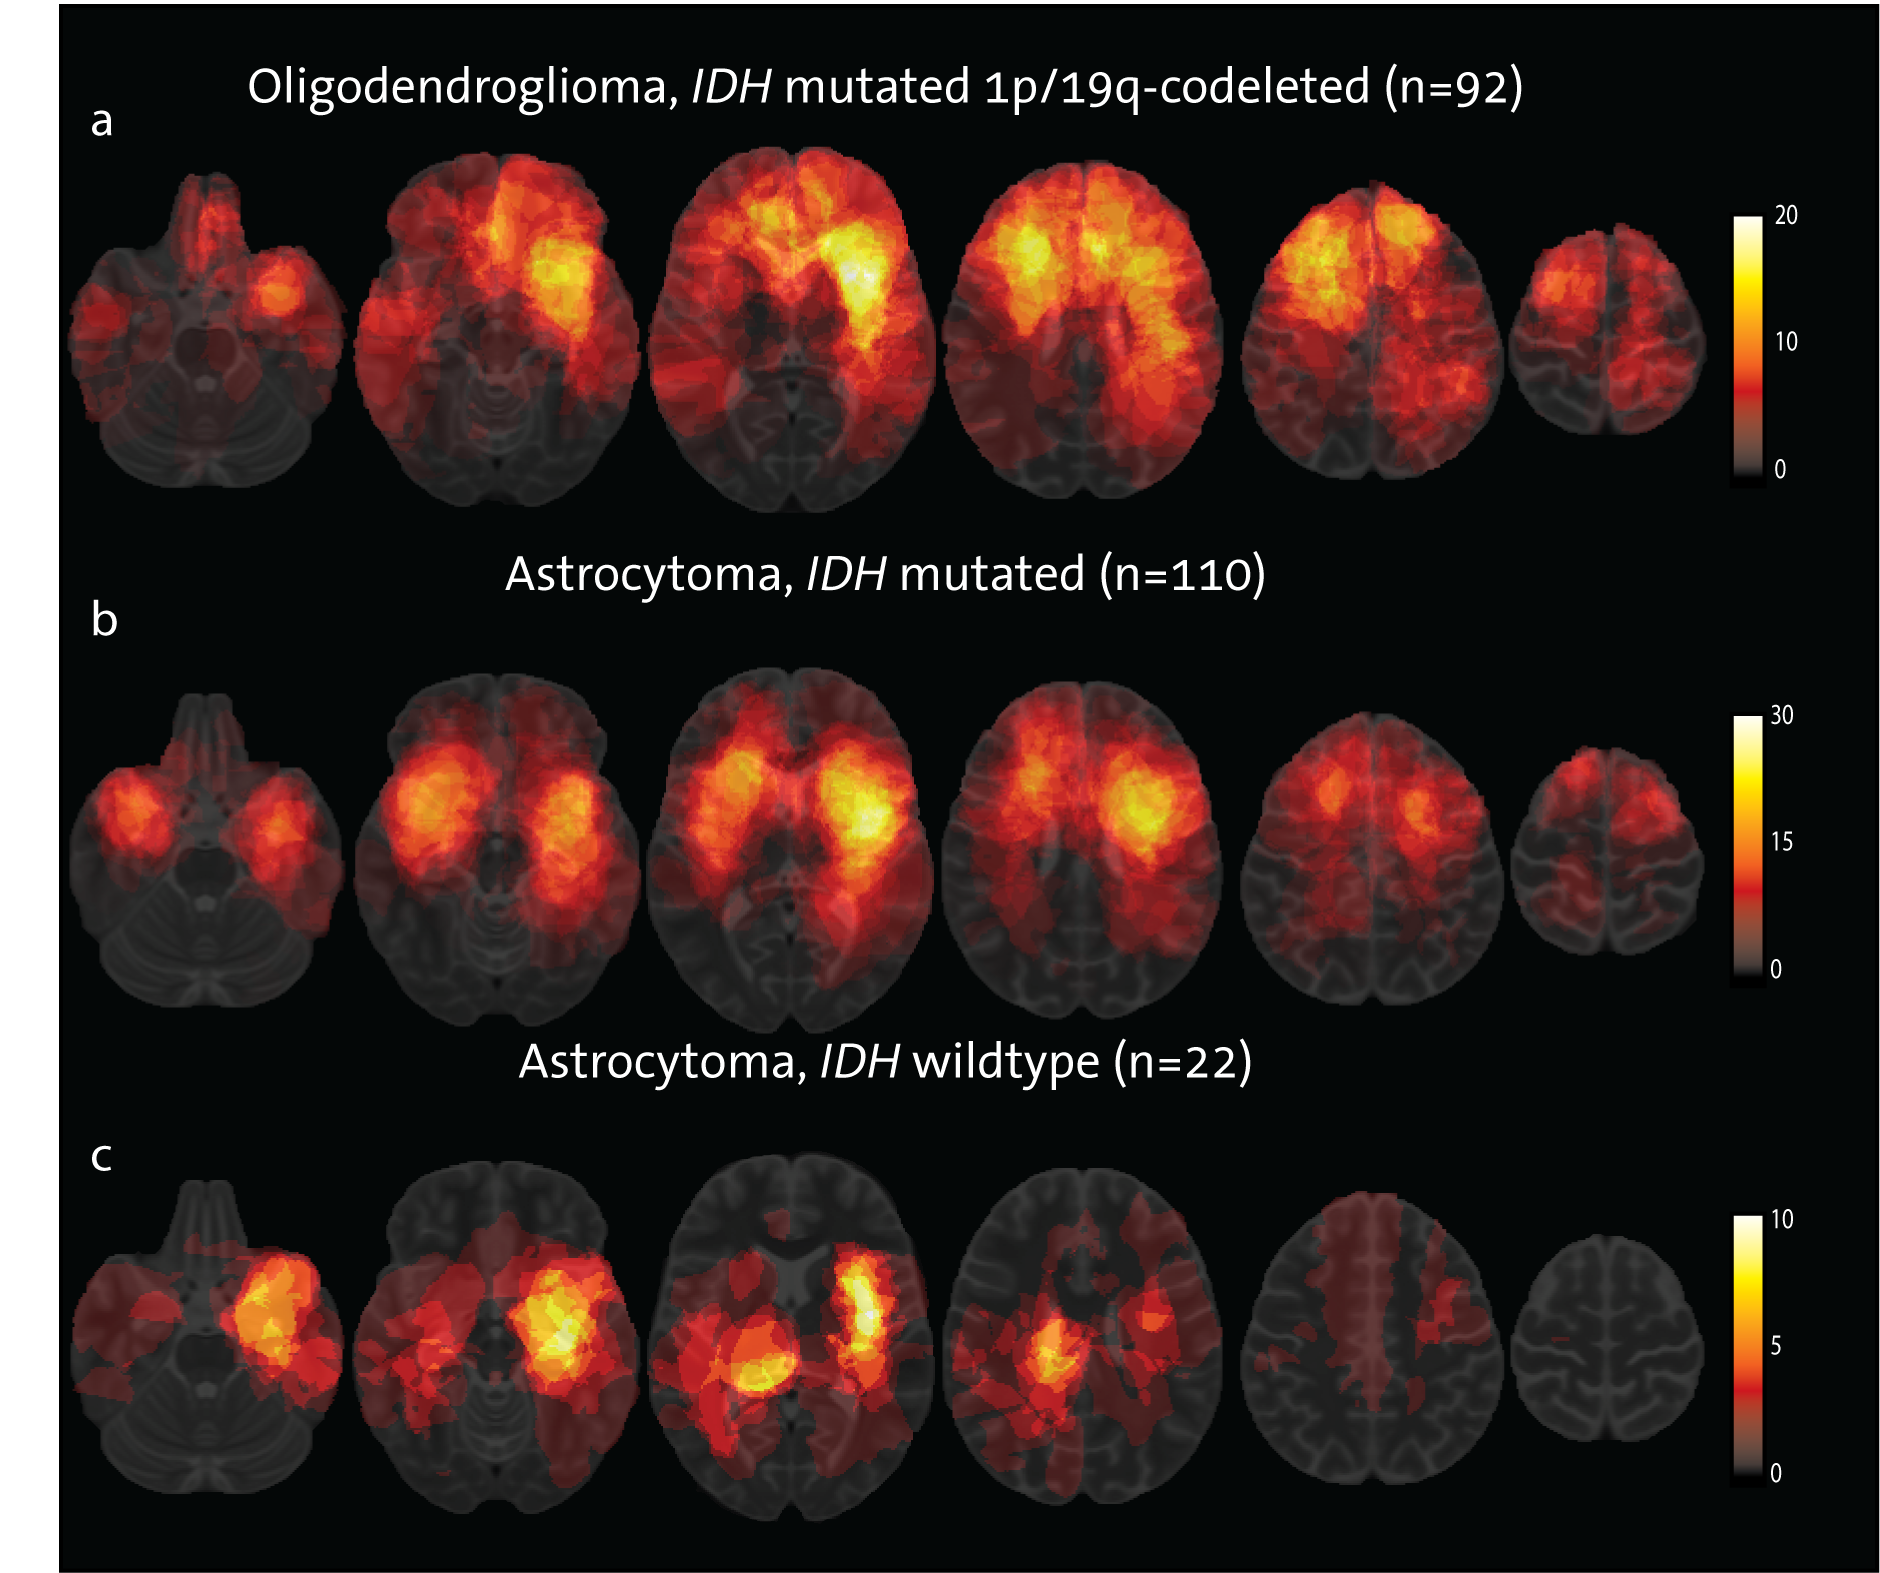
\includegraphics[width=\textwidth]{Figures/Figure_1.png}
\caption{Spatial distribution heatmaps of WHO 2016 glioma subgroups. The color of a voxel corresponds with the number of tumors localized at that
location, ranging from red (low number) to white (high number). The color bars on the right indicate the frequencies corresponding with the color
per voxel; (a) location distribution of oligodendroglioma shows most are located in the frontal lobes. (b) IDH-mutated astrocytoma shows a distri-
bution with most tumors located in or near the insular region. (c) IDH wild-type astrocytomas are more often located in midline region and basal
ganglia.}
\label{fig:LGG_location_heatmap_subgroups}
\end{figure}


\begin{figure}
\centering
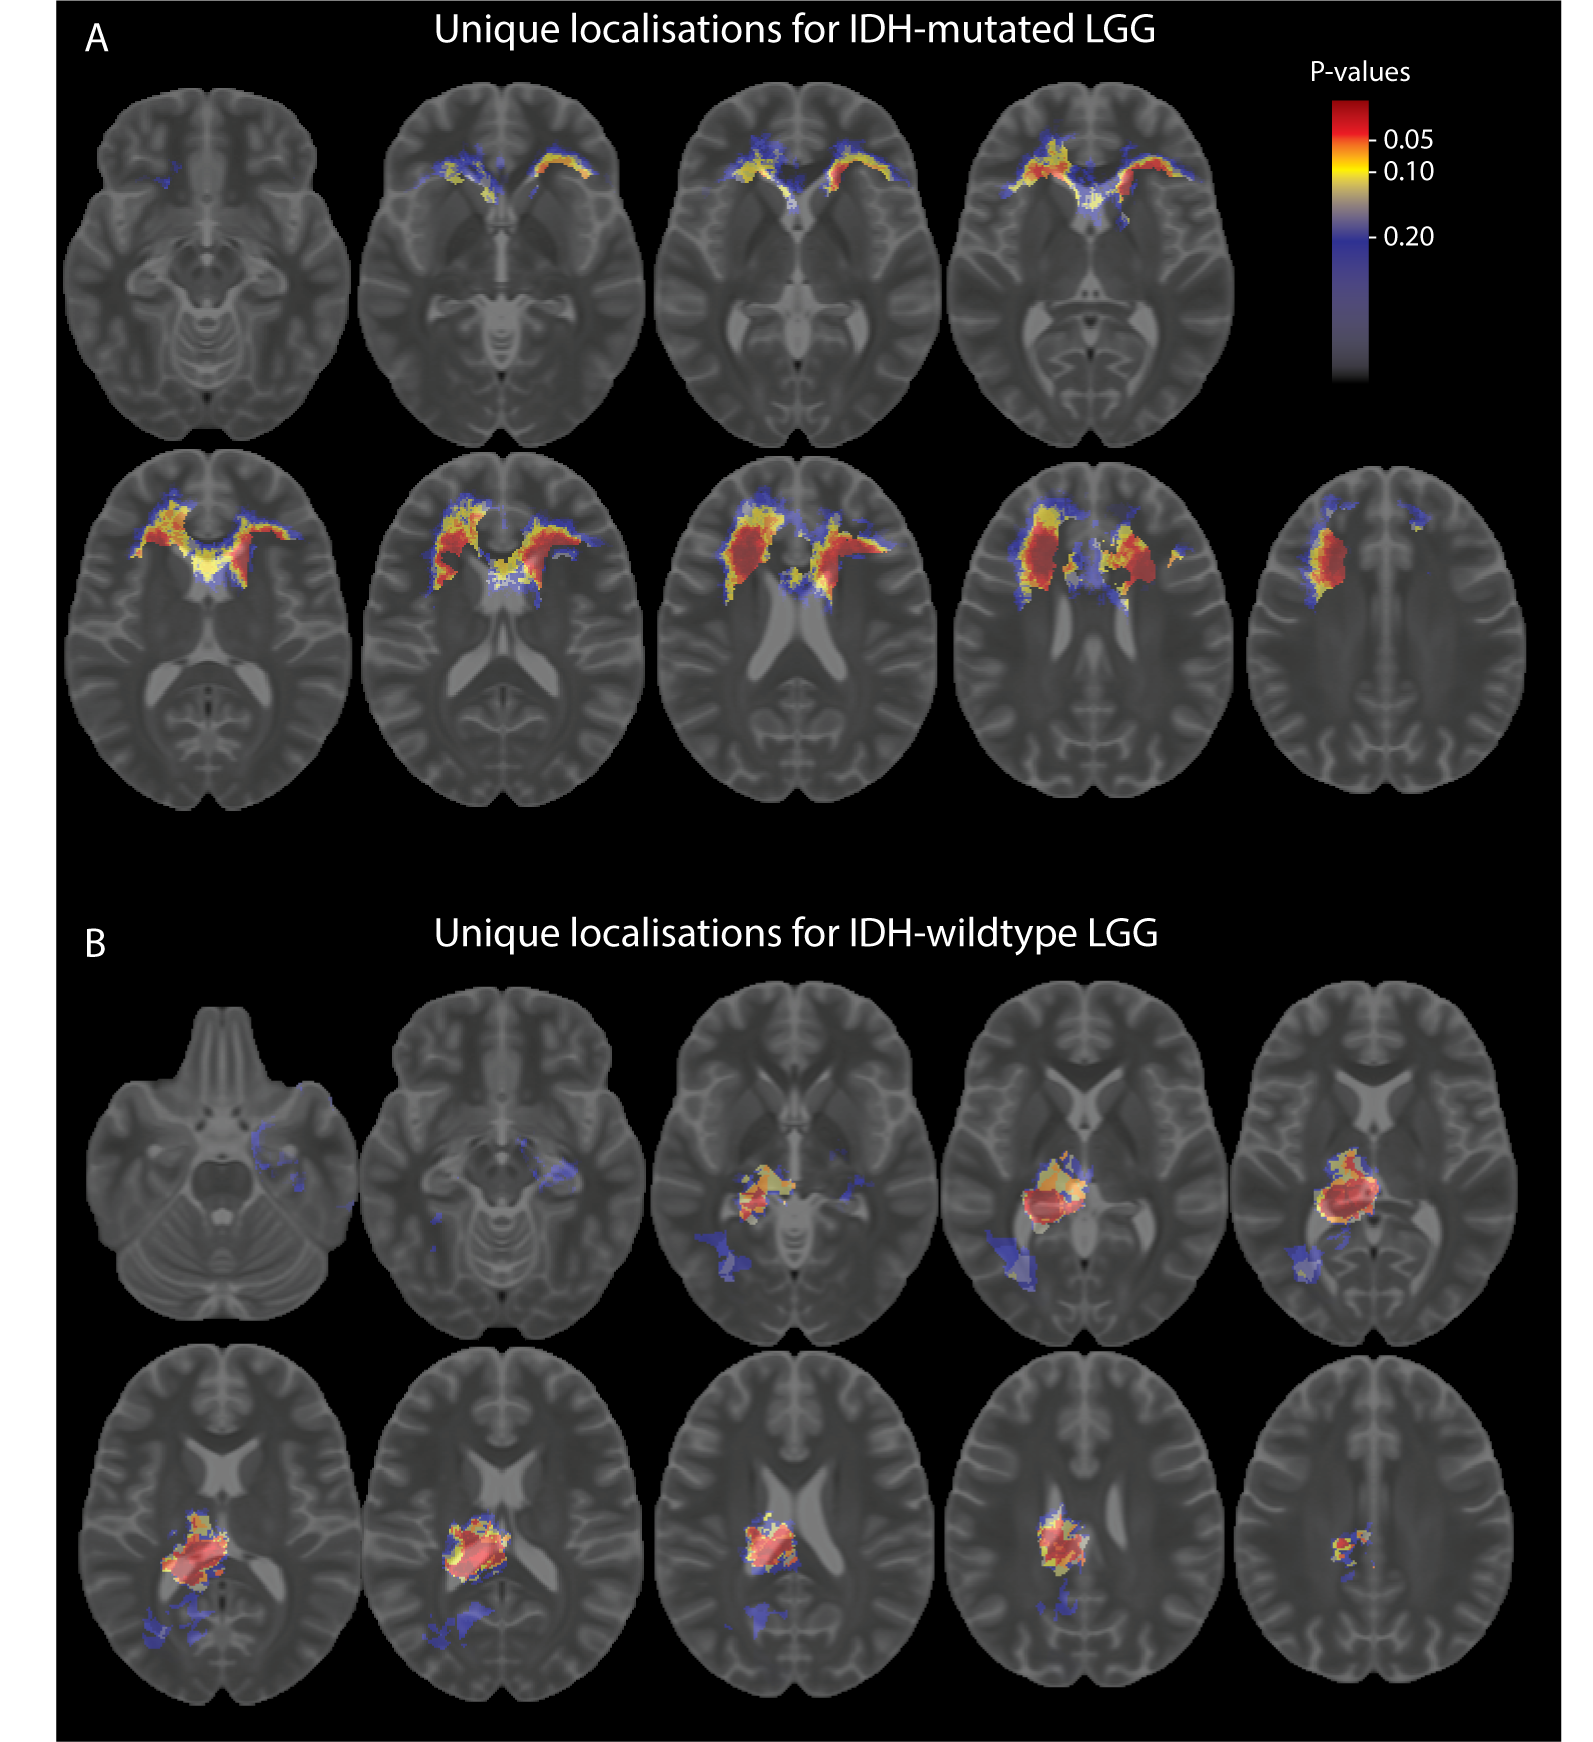
\includegraphics[width=\textwidth]{Figures/Figure_2.png}
\caption{Differences in location distribution between \cgls{IDH} wild-type and mutated low-grade gliomas. Voxel-color indicates corrected P-value with
color bar for scale; (a) regions more often occupied by \cgls{IDH}-mutated low-grade gliomas; (b) regions more often occupied by \cgls{IDH} wild-type low-
grade gliomas.}
\label{fig:LGG_location_P_values}
\end{figure}

\subsection{Exploratory Analysis of Location Predilection of a Single Gene and CNVs}

As an exploratory analysis, we also generated spatial distribution heatmaps of the additional genes and \cglspl{CNV} we tested with our dedicated \cgls{NGS} panel that were frequently mutated or aberrant.
For this, we analyzed CIC and FUBP1 mutations, and loss of chromosomal arm 9p for oligodendroglioma (Supplementary Figure 2).
We found no preferential locations for any of those molecular aberrations, except for loss of 9p (compared with oligodendroglioma with intact 9p), which seemed to be more frequently located in the left parietal area (Supplementary Figure 3).

In \cgls{IDH}-mutated astrocytoma, we created heatmaps of loss of chromosomal arm 9p and imbalance of chromosome 7, and found no preferential brain locations/voxels for either of those that showed P-values $<$0.05 (Supplementary Figure 4).

\subsection{Resection Pobability of LGG}
For a previous study on the extent of resection in the same cohort, postoperative tumor volumes were also assessed with the BrainLab Elements SmartBrush Tool.
We assigned patients into one of the 4 groups based on the postoperative tumor volume: 0.0, 0.1-5.0, 5.1-15.0, and $>$ 15.0 cm$^3$ postoperative tumor volume.
We generated location distribution heat maps stratified by these 4 groups, to investigate if there are preferential localizations for gross total resections.
Results are shown in Figure 3.
All tumors with a total resection (0.0 cm$^3$ postoperative residue) were located in the frontal lobe.
Similarly, the majority of tumors with a low postoperative tumor volume (0.1-5.0 cm$^3$) were located in the frontal lobes.
Tumors with a postoperative volume of more than 5.0 cm$^3$ more frequently occurred in the insular region, temporal lobes, and in or near the primary sensory and motor cortex.

\begin{figure}
\centering
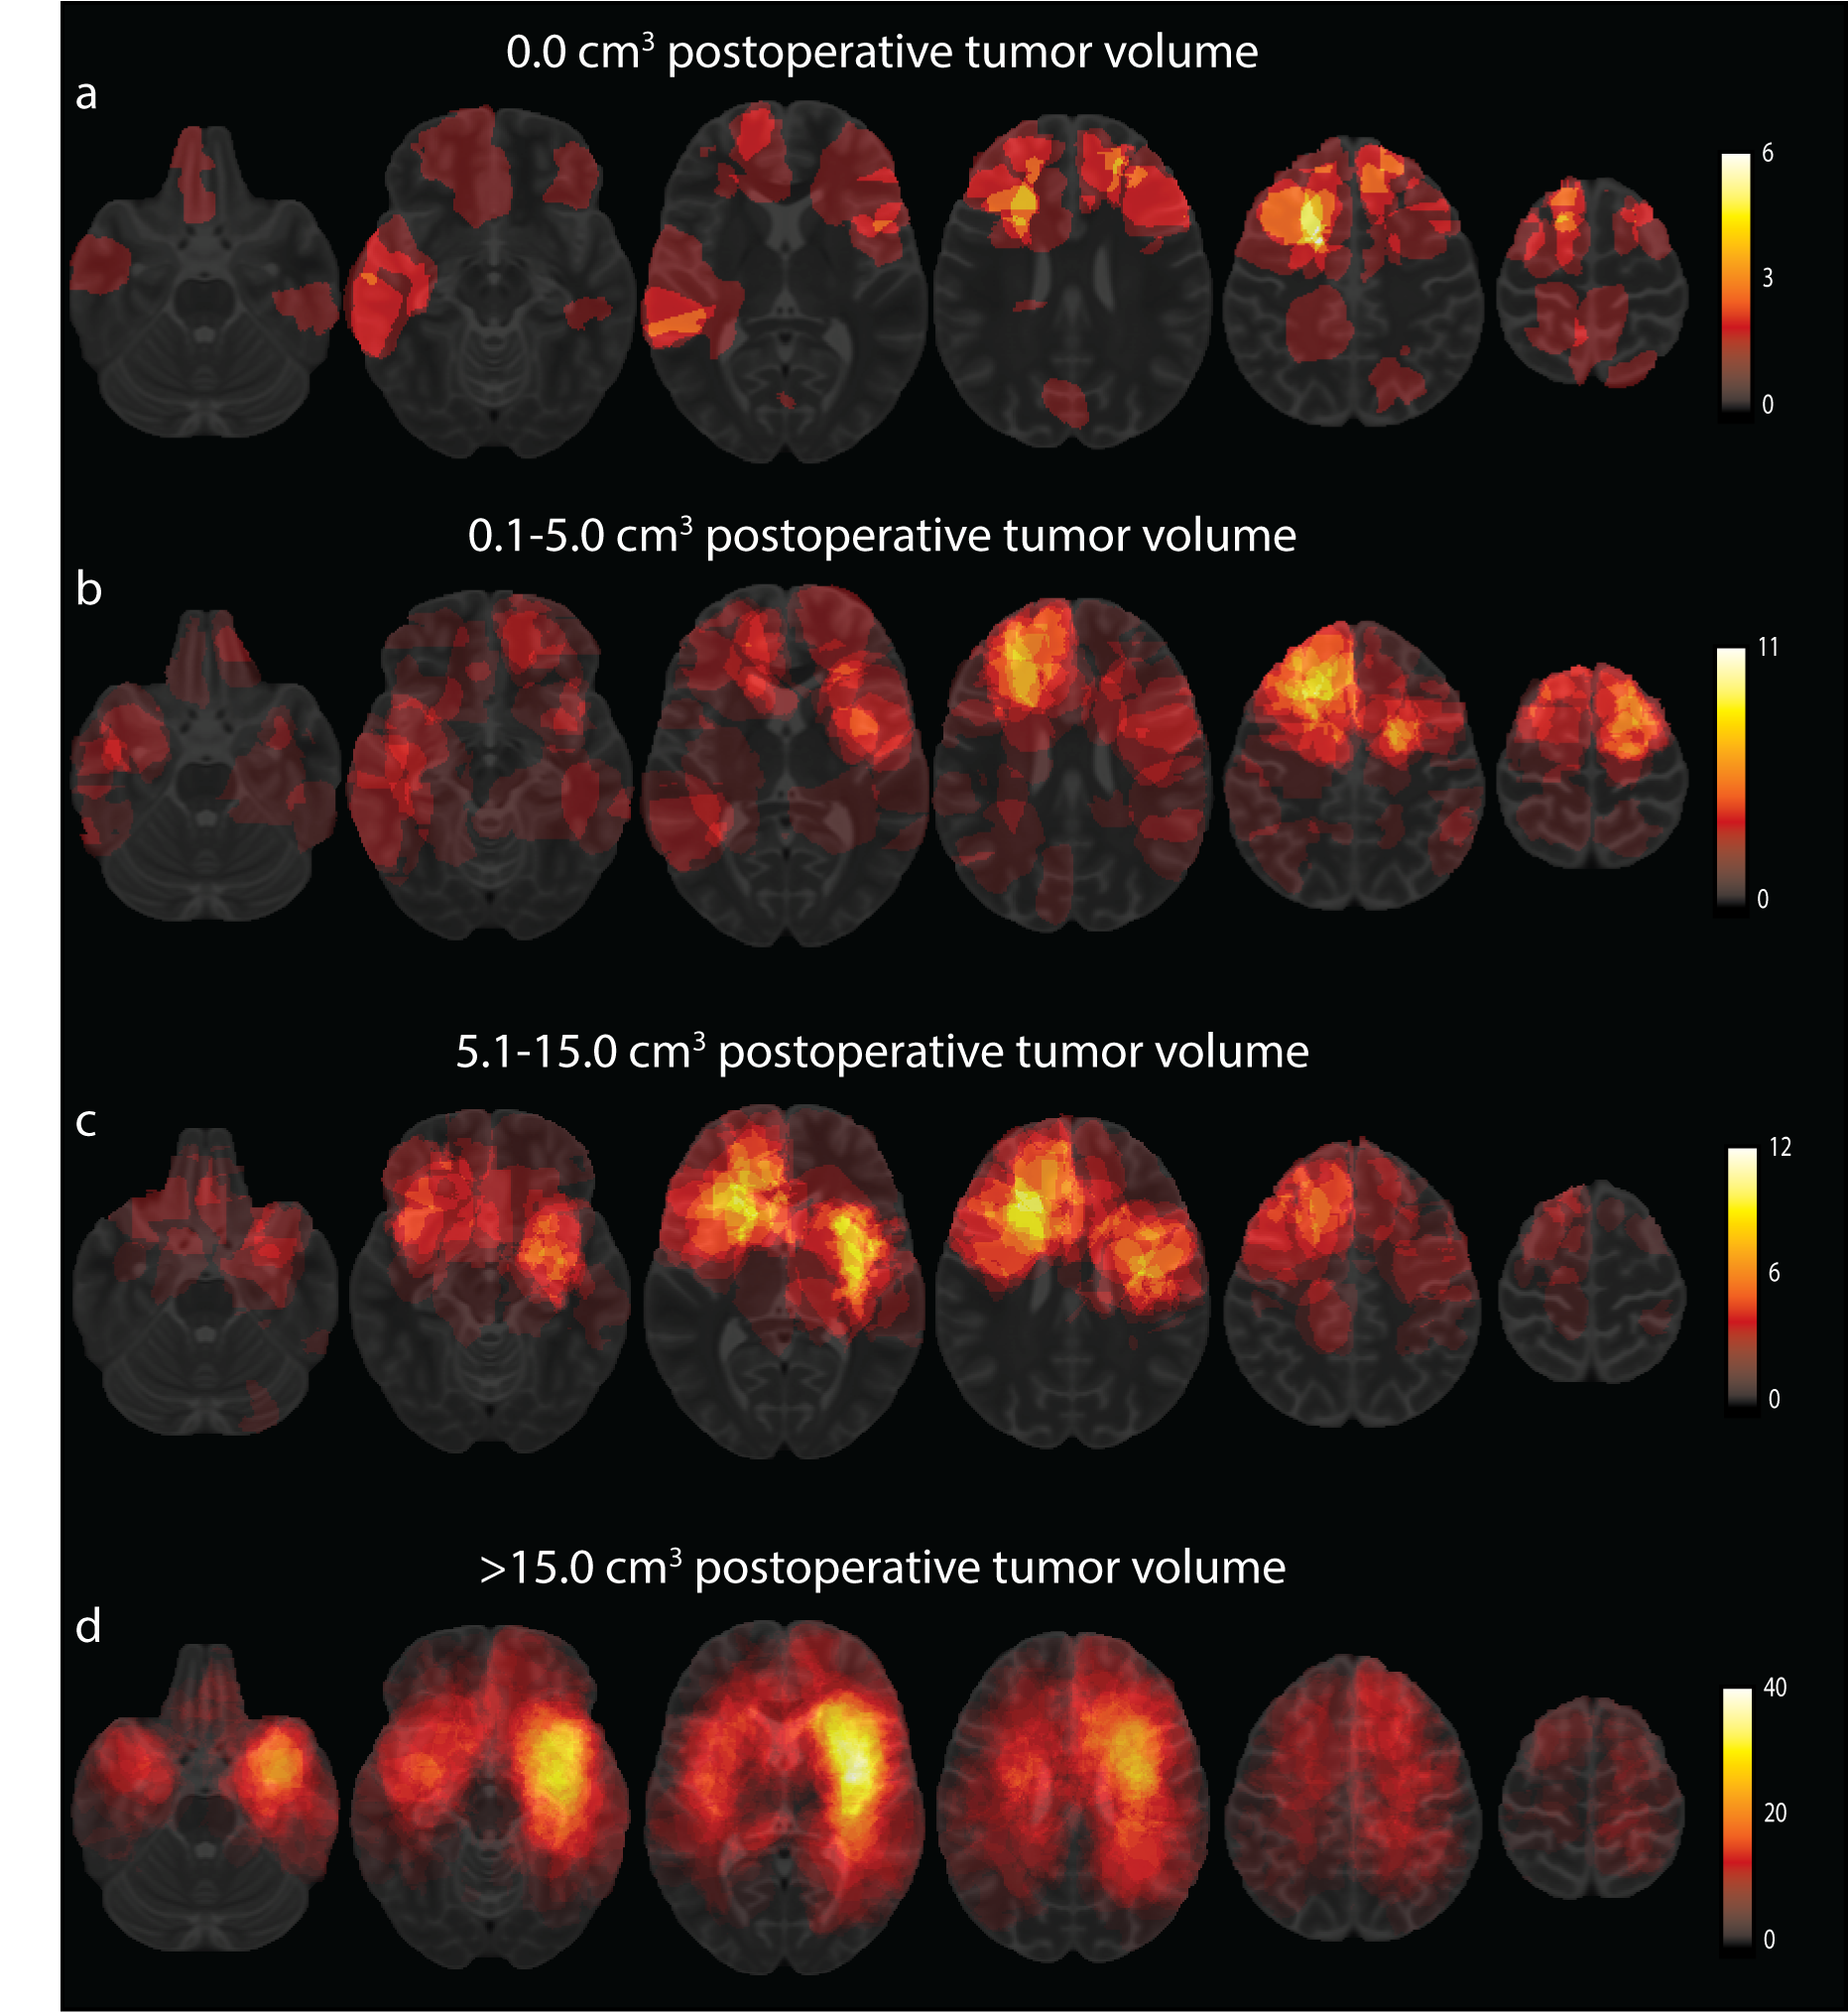
\includegraphics[width=\textwidth]{Figures/Figure_3.png}
\caption{Spatial distribution heatmaps of \cgls{WHO} 2016 grade II glioma stratified according to postoperative tumor volume. The color bars on the right
indicate the frequencies corresponding with the color of the voxels; (a) gliomas with a total resection (0.0 cm$^3$ residue); (b) gliomas with a postop-
erative tumor volume of 0.1-5.0 cm$^3$ ; (c) gliomas with a postoperative tumor volume of 5.1-15.0 cm$^3$ ; (d) gliomas with a postoperative tumor volume
of more than 15.0 cm$^3$.}
\label{fig:LGG_location_postop_volume}
\end{figure}


\section{Discussion}
In this study, we aimed to visualize and compare the spatial distribution of \cgls{WHO} 2016 grade II glioma subgroups.
By using advanced image processing analyses, we were able to generate accurate spatial distribution maps, especially compared with previous studies that were primarily based on location description/scores \autocite{stockhammer2012idh1, goze2009lack, laigle2004correlations, metellus2010absence}.
Our data indicate there are significant differences in spatial distribution patterns dependent on \cgls{IDH} status, with \cgls{IDH}-mutated \cglspl{LGG} more frequently located in the rostral extensions of the lateral ventricles, and \cgls{IDH} wild-type astrocytomas more frequently in the basal ganglia of the right hemisphere.
Our data are in line with earlier observations and confirm there is a correlation between molecular background of a glioma and anatomic location \autocite{stockhammer2012idh1, goze2009lack, laigle2004correlations, metellus2010absence, tejada2018voxel}.
On the other hand, our data also indicate an overlap in anatomic location between \cgls{WHO} 2016 subgroups.

Upon visual inspection, a distinct pattern is clearly recognized between groups: most oligodendrogliomas are located in the frontal lobes and cortex, while \cgls{IDH}-mutated astrocytomas are more frequently located in the frontotemporal and insular region.
However, the substantial overlap between \cgls{IDH}-mutated astrocytomas and oligodendrogliomas can be appreciated as well.
This is also indicated by our voxel-cluster-based statistical analysis, wherein we find a significant predilection for \cgls{IDH}-mutated \cglspl{LGG} in the rostral extensions of the anterior lateral ventricles (\cgls{IDH}-mutated astrocytomas and oligodendrogliomas grouped together), while we could not find regions significantly associated with either \cgls{IDH}-mutated astrocytomas or oligodendrogliomas when we analyzed them as individual entities.
Although oligodendrogliomas and \cgls{IDH}-mutated astrocytomas differ in clinical behavior (overall survival, sensitivity to chemotherapy) and are recognized as independent entities by the \cgls{WHO} classification, both entities share the \cgls{IDH} mutation.
It is suggested that the cell of origin for \cgls{IDH}-mutated gliomas is localized within the subventricular zone \autocite{sanai2005neural}.
If oligodendrogliomas and \cgls{IDH}-mutated astrocytomas share the cell type of origin, this might explain the significant predilection of \cgls{IDH}-mutated \cglspl{LGG} in the rostral extensions of the anterior lateral ventricles, and the absence of a location difference between \cgls{IDH}-mutated astrocytomas and oligodendrogliomas.

Compared with \cgls{IDH}-mutated \cglspl{LGG}, \cgls{IDH} wild-type astrocytomas showed a distinct spatial distribution with more lesions located in the midline and basal ganglia.
This different spatial distribution is an interesting observation, as it shows that, in the setting of grade II gliomas, \cgls{IDH} wild-type astrocytomas have a different anatomical and thus clinical presentation.
The spatial distribution explains the high percentage of biopsies in these patients we reported previously, as tumors in these locations are not eligible for safe resections \autocite{wijnenga2017impact}.
We also reported previously \autocite{wijnenga2017impact} that these tumors often do not present with epilepsy, in contrast to \cgls{IDH}-mutated grade II gliomas, and this might also be explained by their preferential, noncortical location.
On the other hand, it has also been postulated that high frequency of epilepsy in \cgls{IDH}-mutated gliomas is explained by mimicking the activity of glutamate on the NMDA receptor due to high levels of d-2-hydroxyglutarate \autocite{chen2017mutant}.

Upon visual inspection in this series, both oligodendrogliomas and \cgls{IDH}-mutated astrocytomas were slightly more frequently located in the left hemisphere, especially in insular location.
An explanation might be a selection bias of patient referral because our center was one of the first in the Netherlands that performed awake craniotomies, which are performed for tumors located in presumed eloquent regions such as the left insular, frontal, and temporal region.

A current hot topic in glioma research is the development of noninvasive prediction of \cgls{WHO} 2016 classification of tumor diagnosis based on preoperative MR scans.
This would be very helpful for presurgical decision-making.
In a previous study, for example, we showed that minor postoperative tumor residues have more impact on survival in \cgls{IDH}-mutated astrocytomas than in oligodendrogliomas \autocite{wijnenga2017impact}.
Our data show that anatomic location could contribute to this noninvasive prediction, but requires the combination with other parameters to predict \cgls{WHO} subtype accurately.

We performed an exploratory analysis to assess the spatial distribution of other frequently reported mutations and \cglspl{CNV} in glioma.
Potential differences in spatial distribution might generate hypotheses or clues about the origin of glioma or specific subgroups and aggressiveness of certain glioma subtypes.
We found no specific spatial distributions for the tested aberrations however, except for loss of chromosome 9p in the context of oligodendroglioma.
Oligodendrogliomas with loss of 9p were significantly more frequently located in the left parietal area.
This finding needs to be confirmed in independent series before any assumptions regarding the relevance on the biological level can be made.

As a second aim we visualized the possible correlation between anatomic location of \cgls{LGG} and the extent of their resection.
State-of-the-art neurosurgical techniques including awake craniotomies were used in this cohort to achieve resections as extensive as possible in a safe way.
Upon visual inspection, we found that \cglspl{LGG} with no or very small postoperative tumor residues (more extensive resections) were more frequently located in the frontal lobes, while \cglspl{LGG} with larger postoperative tumor volumes were more frequently located in the insular and temporal regions.
This is an expected result, as the extent of resection is associated with anatomic location and also with proximity of eloquent areas of the brain \autocite{wijnenga2017impact}.
Our heatmaps provide an insightful visualization which might be helpful in surgical planning and in informing patients on resectability of an \cgls{LGG}.

Our study has several contributions compared with previous studies.
We used a relatively large and representative consecutive cohort of \cglspl{LGG}, which were all classified with \cgls{NGS} according to the integrated \cgls{WHO} 2016 criteria.
To the best of our knowledge, this is the first study that visualizes the spatial distribution of gliomas classified according to the \cgls{WHO} 2016 classification.
Also, we scored location in a voxel-based manner with the use of semi-automated segmentation software, which gives a far more accurate representation of location compared with a manual scoring of location.
Some limitations have to be addressed as well.
Our study was retrospective in nature, and the \cgls{MRI} protocols were not standardized.
Consequently, voxel size and slice thickness were not homogeneous in the cohort.
Images with large voxel size and slice thickness pose challenges for accurate segmentation and registration.
More subtle differences in location between groups might be missed.
However, our aim was not to find subtle differences, but clinically relevant differences between groups, and our cohort with heterogeneous \cgls{MR} protocols is sufficient for this aim (and also reflects the 'real-life' situation).
More importantly, the mapping of patient \cgls{MR} scans with segmentation to the \cgls{MNI} standard brain can lead to distortion and a slight change of location on the standard brain compared with the original \cgls{MR} scan.
This is especially relevant for relatively large lesions with mass effect, for example, tumors that compress the ventricles.
Because of this, our heatmaps erroneously showed some tumors to be located in the ventricles.
However, if a registration that perfectly mapped the tumor to its position along the ventricle (instead of mapping it inside the ventricle), the tumor would have been compressed.
As such the resulting mapping would misrepresent the actual tumor volume.
Therefore, we have chosen to accept the erroneous mappings into the ventricles in favor of these volume effects.
To be as accurate as possible, we manually checked all registrations and corrected where necessary.
Furthermore, although this is a relatively large consecutive series of molecular-defined grade II glioma, a further expansion of our dataset is needed, as especially the group of \cgls{IDH} wild-type astrocytomas is small.
We need larger numbers to confirm that the spatial distribution of \cgls{IDH} wild-type \cgls{LGG} is indeed different compared with \cgls{IDH}-mutated \cgls{LGG}, as it is known that glioblastomas are also frequently located in the frontal lobes.
However, a recent study showed that, in the context of glioblastoma, the frontal cortex is also significantly associated with the presence of \cgls{IDH} mutations \autocite{tejada2018voxel}.

In conclusion, \cgls{WHO} 2016 low-grade glioma molecularly defined subgroups show both differences and similarities in spatial distribution, with \cgls{IDH}-mutated \cglspl{LGG} significantly more frequently located in the frontal lobes and \cgls{IDH} wild-type tumors more frequently in the basal ganglia of the right hemisphere.

\newpage
\begin{subappendices}
    \section{Supplemental Figures}

    \begin{figure}[htb]
        \centering
        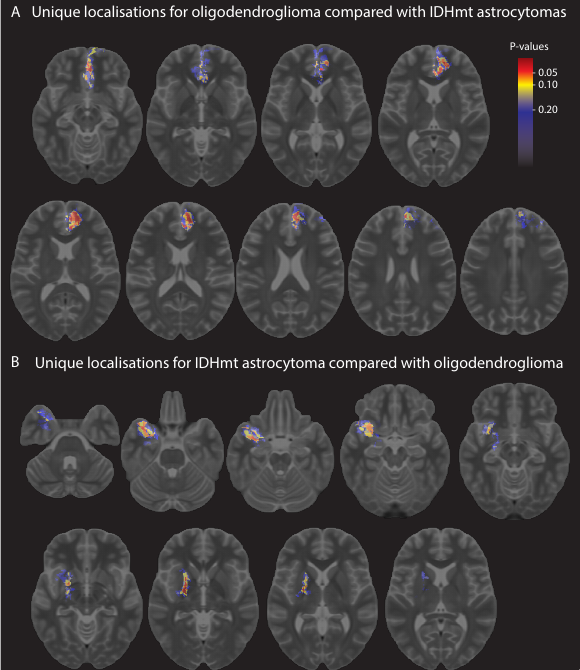
\includegraphics[width=\textwidth]{Figures/p_value_oligo_astro.png}
        \caption{Results of the FSL Randomize test with 15000 permutations for statistical
        differences in location distribution. The color of a voxel is correlated with
        a p-value as indicated in the top-right color bar; (a) heatmap of unique
        localisations for oligodendroglioma compared with IDH mutated astrocytomas (b) heatmap of unique localisations for IDH mutated astroctyomas
        compared with oligodendrogliomas}\label{fig:LGG_location_oligo_astro_p_value}
    \end{figure}

    \begin{figure}[htb]
        \centering
        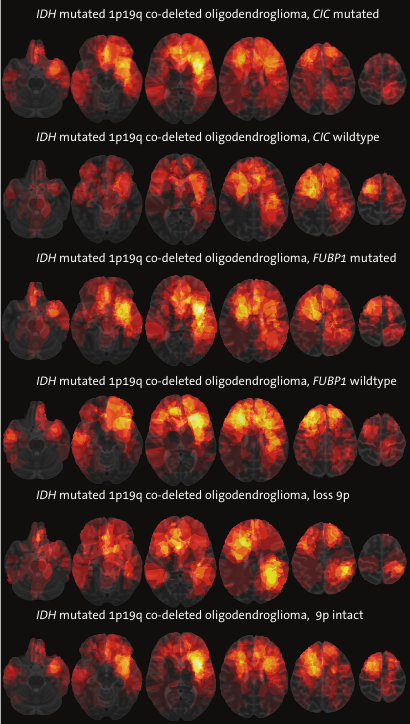
\includegraphics[height=\textheight]{Figures/heatmap_multi_parameter.png}
        \caption{Spatial distribution heatmaps of presence of individual gene or copy number alterations in the context of oligodendroglioma}\label{fig:LGG_location_heatmap_multi_genetics}
    \end{figure}

    \begin{figure}[htb]
        \centering
        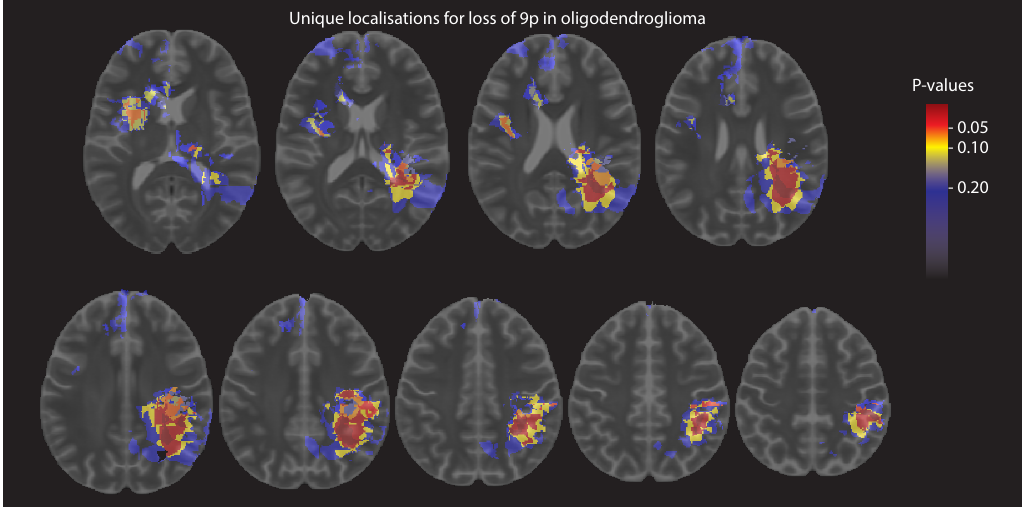
\includegraphics[width=\textwidth]{Figures/p_value_9p.png}
        \caption{Results of the FSL Randomize test showing unique localisations for loss of 9p in the context of oligodendroglioma}\label{fig:LGG_location_p_value_9p}
    \end{figure}
\end{subappendices}
